\documentclass[amsmath,amssymb,twocolumn,superscriptaddress]{revtex4-1}

\usepackage{graphicx}% Include figure files
\usepackage{dcolumn}% Align table columns on decimal point
\usepackage{bm}% bold math
\usepackage[detect-all]{siunitx}
\usepackage{hyperref}% add hypertext capabilities
\usepackage{xr}

\begin{document}                  % DO NOT DELETE THIS LINE

\title{Introducing classical molecular dynamics simulation to users of
scattering}

\author{A.~R. McCluskey}
\email{a.r.mccluskey@bath.ac.uk}
\affiliation{Department of Chemistry, University of Bath, Claverton Down,
Bath, BA2 7AY, UK}
\affiliation{Diamond Light Source, Harwell Campus, Didcot, OX11 0DE, UK}

\author{J. Grant}
\affiliation{Computing Services, University of Bath, Claverton Down, Bath, BA2 7AY, UK}

\author{A.~R. Symington}
\affiliation{Department of Chemistry, University of Bath, Claverton Down,
Bath, BA2 7AY, UK}

\author{T.~Snow}
\affiliation{Diamond Light Source, Harwell Campus, Didcot, OX11 0DE, UK}
\affiliation{School of Chemistry, University of Bristol, Bristol, BS8 1TS, UK}

\author{J.~Doutch}
\affiliation{ISIS Facility, Rutherford Appleton Laboratory, STFC, Chilton, Didcot, OX11 0QX, UK}

\author{B.~J. Morgan}
\email{b.j.morgan@bath.ac.uk}
\affiliation{Department of Chemistry, University of Bath, Claverton Down,
Bath, BA2 7AY, UK}

\author{S.~C. Parker}
\affiliation{Department of Chemistry, University of Bath, Claverton Down,
Bath, BA2 7AY, UK}

\author{K.~J. Edler}
\email{k.edler@bath.ac.uk}
\affiliation{Department of Chemistry, University of Bath, Claverton Down,
Bath, BA2 7AY, UK}

\date{\today}

\begin{abstract}
\noindent Classical molecular dynamics simulations are rapidly becoming a popular component of multi-modal analyses from scattering measurements; such as small angle scattering and diffraction.
However, few users of these techniques have formalised training in these methodologies, resulting in frequent use of molecular dynamics simulations as a black box technique.
This work discusses an open educational resource designed to introduce classical molecular dynamics to users of scattering, describing possible sources of error in the method.
Furthermore, we cover some of the methods that can be used to enable simulation techniques to facilitate the analysis of scattering data.
\end{abstract}

\maketitle                        % DO NOT DELETE THIS LINE

\section{Introduction}

\noindent The use of molecular dynamics simulations to aid in the analysis of experimental data, particularly from small angle scattering (SAS) and diffraction, has grown significantly over the past ten years \cite{pan_molecular_2012,boldon_review_2015,hub_interpreting_2018,ivanovic_temperature-dependent_2018,east_structural_2016,wall_conformational_2014,wall_internal_2018,satoh_multiple_2015}.
Figure \ref{fig:growth} shows the growth in the percentage of SAS publications that mention molecular dynamics.
It can be seen that there has been a linear growth in such publications, with more than \SI{20}{\percent} of all SAS publications mentioning molecular dynamics as of 2018.
This alone is a clear indication of the importance that simulation techniques are having on the field of scattering and diffraction.

Normally, the users of scattering and diffraction techniques have a background in experimental science, with little or no formalised training in computational modelling techniques.
This may be problematic, as it can lead to the use of molecular simulation as a black-box, with little understanding or consideration for the underlying methodologies.
The use of molecular simulations in this fashion can quickly lead to the inclusion of severe, systematic errors.
This has lead to the development of tools, such as WAXSiS or SASSIE \cite{chen_validating_2014,knight_waxsis_2015,perkins_atomistic_2016}, that present easy-to-use interfaces designed to reduce the risk of these errors.

In addition to the development of software packages, another method to further limit systematic errors consists of lectures or workshops presenting an introduction to molecular simulation for scattering and diffraction users.
For example, the annual ISIS Neutron Training Course now includes a module entitled ``An Introduction to Molecular Dynamics for Neutron Scattering''.
This details the fundamentals of classical molecular dynamics simulation, before presenting applications of these methods in neutron science, in turn, allowing students an opportunity to gain familiarity with the SASSIE software package \cite{perkins_atomistic_2016}.
While such lectures and workshops comprise an important aspect of training, they are limited in terms of the numbers of students that may attend and the course's location.
Ultimately this means that not all scattering and diffraction users may easily access such resources.

%
\begin{figure}
\label{fig:growth}
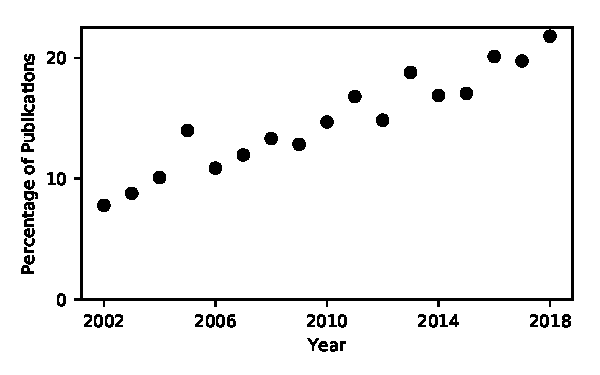
\includegraphics[width=0.48\textwidth]{figures/chem_data_py.pdf}
\caption{The annual growth of the percentage of publication that mention ``small angle scattering'' which also mention ``molecular dynamics''. Determined from the number of results from a Google Scholar search.}
\end{figure}
%

There has been a recent movement within the scientific and engineering communities towards technology-enhanced open educational resources (OERs).
These are courses, lectures, or learning resources that are made freely available online for use by anyone.
This allows the permission for others to engage in the ``5R activities'': Retain, Reuse, Revise, Remix, and Redistribute \cite{wiley_open_2018}.
The act of publishing an OER increases the reach of a particular resource as it allows others to pick it up, modify it, and use the modified version in their own teaching.
The availability of the Jupyter Notebook framework \cite{kluyver_jupyter_2016} has facilitated the availability of OERs by improving the ability for students to interact directly with the resource often, but not always, using the Python programming language \cite{barba_cybertraining_2017}.

Herein, we present an online, open-source, interactive learning resource aimed to introduce members of the scattering and diffraction community to molecular dynamics simulations.
This open educational resource comprises of six lessons, covering classical methods, introducing molecular dynamics, and showing how this method may interact with scattering in a multi-modal fashion.
We leverage the open-source Python library \texttt{pylj} \cite{mccluskey_pylj_2018} to give a visual and programmatic representation of the interactions between these two techniques.
In this paper, we will discuss the implementation of the resource and detail how the student may get the most from the resource (in this work \emph{the student} refers to anyone working through the OER, regardless of career position).

\section{Assumed prior knowledge}

The OER, entitled \emph{``The interaction between simulation and scattering''} makes use of the Python programming language, this allows for interactive examples of the mathematical and algorithm content to be included.
A result of this is that to be able to fully utilise the resource some knowledge of, or willingness to learn, Python is required.
However, we have attempted to develop the resource in such a fashion that an in-depth knowledge of Python is not required.
It is anticipated that the users of this resource would have some familiarity with undergraduate level chemistry or physics, alongside a commensurate understanding of mathematics.
This is particularly important when considering the nature, and chemical rationale, of classical interaction potentials.

\section{Resource construction}

The resource is currently available online, at \url{https://pythoninchemistry.org/sim_and_scat} \cite{mccluskey_pythoninchemistry/sim_and_scat_2019}.
These web pages were written as a series of Jupyter Notebooks and Markdown files, which were then compiled using the jupyter-book functionality \cite{lau_jupyter/jupyter-book_2019}.
The use of this system allows for Python code blocks to be included alongside the textual content providing algorithmic details whilst also facilitating interactivity, though both Thebelab and BinderHub integrations \cite{ragan-kelley_minrk/thebelab_2019,ragan-kelley_jupyterhub/binderhub_2019,jupyter_binder_2018}.
Interacting with the resource in this fashion will allow the student to either run the Python code directly in the resource interface (Thebelab) or easily launch a MyBinder window to more intensive visualisations (such as \texttt{pylj}).

The resource is provided under a CC-BY-SA-4.0 license \cite{noauthor_creative_2019} and builds on the growing library of open educational resources.
The open-source nature of this license means that anyone may use the material to enhance their own educational platform and experts in the field may contribute to improving the resource.
The source code for the resource is available at \url{https://github.com/pythoninchemistry/sim_and_scat} \cite{mccluskey_pythoninchemistry/sim_and_scat_2019}.

\section{Resource outline}

The resource follows a simple outline to introduce important aspects of molecular dynamics simulations.
Code blocks are used to gradually build up the student's understanding of the various concepts.

\subsection{Home}

The welcome page introduces the resource and gives the student information about how the resource may be used, including details of Thebelab and BinderHub integration.
Furthermore, this page gives information about the use and sharing of the content of the resource including details of the license.
This page also includes an authors and contributors list.

\subsection{Classical methods}

Following the introduction, concepts relating broadly to classical simulation methods are introduced.
This includes the functional nature of potential modelling and gives some examples, such as the Lennard-Jones and Buckingham potential models \cite{lennard-jones_determination_1924,buckingham_classical_1938}.
The potential model parameterisation is briefly covered including the use of higher accuracy quantum mechanical calculations to do so.
The presence of off-the-shelf, general potential models are discussed; with particular attention paid to the caveat that they may still require system specific optimisations.
Finally, we mention mixing rules; again discussing the possible problems that a user may encounter related to system specificity.

\subsection{Molecular dynamics}

Building on the classical potential model methods the student is then presented with molecular dynamics.
This is shown by using different aspects for the method to gradually build up a one-dimensional molecular dynamics simulation using NVE (Number, Volume and Energy) ensembles, the Velocity-Verlet algorithm and the Lennard-Jones potential model \cite{swope_computer_1982,lennard-jones_determination_1924}.
This is introduced in terms of Newton's laws of motion and the generalised equations of motion, which should be familiar to most students.
Finally, different importance considerations for molecular dynamics simulations are described including ensembles, the potential cut-off, and periodic boundary conditions.

\subsection{\texttt{pylj} and the interaction with scattering}

The final aspect of the resource is to utilise a molecular dynamics simulation to understand some scattering profiles.
This is achieved using the open-source \texttt{pylj} package \cite{mccluskey_pylj_2018}, which allows for a two-dimensional simulation or argon particles, interacting through a Lennard-Jones potential, to be performed.
The student is first shown a working \texttt{pylj} simulation and invited to interact with the simulation and the custom plotting functionality of \texttt{pylj}.
In the final lessons, a formulation of the Debye equation \cite{debye_zerstreuung_1915} is given and the student is invited to observe the effect of simulation temperature on the resulting scattering profile.
There is mention of other, faster, algorithms for the determination of scattering profiles, such as the Fibonacci sequence or Golden Vectors methods \cite{svergun_solution_1994,watson_rapid_2013}.

\section{Future outlook}

In the future, we hope that the nature of the material, as an OER, will promote interest from other parties towards reuse, and remixing the material.
Furthermore, we hope to implement this material within training at the ISIS Neutron and Muon Source as well as Diamond Light Source.
Finally, it is hoped, \textit{via} student and community feedback, that the improvement of implementation, materials, and general pedagogy of the resource can be achieved, driving up the quality and depth of molecular dynamics analyses performed on results obtained from scattering and diffraction measurements.

\section{Author contributions}

The open education resource was developed, and the manuscript written, by A. R. M. with input from all authors.

\begin{acknowledgements}
A. R. M. is grateful to the University of Bath and Diamond Light Source for co-funding a studentship (Studentship No. STU0149).
B. J. M. acknowledges support from the Royal Society (Grant No. UF130329).
\end{acknowledgements}

\bibliography{bib.bib}


\end{document}                    % DO NOT DELETE THIS LINE
